\documentclass[12pt,a4paper]{article}

\usepackage{fullpage}
\usepackage[utf8]{inputenc}
\usepackage{amsfonts}
\usepackage{amssymb}
\usepackage[french]{babel}
\usepackage[cyr]{aeguill}
\usepackage{natbib}
\usepackage{graphicx}
\usepackage{tabularx}
\usepackage{hyperref}
\usepackage[document]{ragged2e}
\setlength{\parindent}{2em}
\setlength{\parskip}{1em}

\newcommand{\quotes}[1]{``#1''}

\begin{document}

\begin{titlepage}
\centering
{\scshape\LARGE Université de Bordeaux \par}
{\scshape\Large Master 1 Informatique  \par}
\vspace{3cm}

{\Huge\bfseries Projet de Programmation\par}
{\Huge\bfseries Le Clicodrome de LEFFF \par}
{\Large\bfseries par Lionel CLEMENT \par}
\vspace{0.5cm}
{\Large\itshape Mémoire \par}
{\large 05 Avril 2019\par}

\vfill
réalisé par \par
JELLITE \textsc{Oumayma} \par
BAKIR \textsc{Fatima Ezzahra} \par
NEDELEC \textsc{Guillaume} \par
SYLLA  \textsc{Alfred Aboubacar} \par
\vfill

{\large Enseignants responsables : Philippe NARBEL et Vincent PENELLE\par}

\end{titlepage}

\newpage
\tableofcontents

\newpage\section{Contexte général du projet}
\subsection{Résumé}

\smallbreak Dans ce rapport, nous avons présenté minutieusement notre étude, la conception et le développement d'un site web / Interpréteur :
    \textbf{" Le Clicodrome de LEFFF "}

Pour déterminer les formes fléchies d'un mot en français, notre client Lionel CLEMENT à donc créer un lexique "LEFFF"  contenant un grands nombre de mots de différentes catégories. Cependant, ce lexique est présenter sous format texte qui ne facilite pas l'accès, la modification et l'enrichissement du lexique.
Donc , Nous avons conçu de développer ce site web afin de faciliter l'accès au LEFFF, sa modification et son enrichissement ainsi que la génération des formes fléchies à partir d'un Interpréteur  pour  rendre ce lexique utilisable par n'importe quelle personne qui souhaiterai l'accéder.
Le présent rapport va décrire en détail, les différentes étapes suivies tout au long de ce projet allant de l'étude, 
en passant par la conception et en terminant par la réalisation de l'application.
\subsection{Objectif}
Avant de détailler l’objectif de notre projet, nous allons mettre
au clair quelques notions nécessaires à la compréhension du sujet. 
Il faut savoir que dans la langue française, les formes fléchies d'un mot correspondent à sa conjugaison et à ses déclinaisons (sa forme au pluriel, les mots ayant une correspondance comme "mien" et "moi" par exemple).
De plus ce lexique est un “dictionnaire” contenant un grands nombre de mots de différentes catégories. Ce sont des noms propres, des noms communs, des adverbes, des adjectifs, des tous les autres types de mots possible dans la langue française.
Notre but sera de trier tous ces types de mots afin de déterminer quelles sont les formes fléchies et quelles sont les mots "racines".

Lionel CLEMENT qualifie ce lexique comme "une ressource complexe constituée de
\begin{itemize}
\item Lexème ou grammème (ie Prendre)
\item Vocables (ie Prendre=saisir, Prendre=recevoir)
\item Catégories syntaxiques (ie Verbe)
\item Sous-catégories syntaxiques (ie Transitif, passivable)
\item Catégories grammaticales (ie Nombre$\rightarrow\{sing, plur\}$, Personne$\rightarrow\{1, 2, 3\}$)
\item Règles de flexion (ie Table de conjugaison de prendre - Stem=.*(pren|mett))
\item Valence (ie objet nominal, oblique en à)
\item Réalisation syntaxique (ie passif en par)
\item Phraséologie (ie "Prendre ombrage", "Prendre ses jambes à son cou")
\item Collocation (ie "Prendre une initiative")
\item Fonctions lexicales (ie Magn: "Prendre une belle initiative")
\end{itemize}

L'objectif de ce projet est donc de transformer le lexique au format texte en une base de données et de développer une interface web facilitant les interactions avec ce lexique via cette base de données.
Le projet peut être donc séparé en trois parties principales : 
\begin{itemize}
    \item L'importation du lexique au format texte dans une base de données
    \item La création de l'interface web qui interagira avec la base de données
    \item Le développement d'un compilateur permettant de générer les formes fléchies d"un mot donné en entrée
\end{itemize}
\subsection{Analyse de l'existant}
Pour ce projet, nous avons a notre  disposition différentes versions  du Lefff  dont la dernière réalisé par Benoît Sagot en 2010. Cette version regroupe diffèrent format du lefff , à savoir \cite{lefff_int} :
\begin{itemize}
\item le lexique \textbf{intentionnel}, qui décrit pour chaque entrée son lemme (forme canonique + tableau d'inflexion) ainsi que des informations syntaxiques profondes (cadre de sous-catégorisation profonde + réalisations possibles + restructurations possibles) .
\item le lexique \textbf{extensionnel}, construit automatiquement par compilation du lexique intentionnel. Ce processus de génération comprend une étape d'inflexion, en fonction de la classe d'inflexion associée à l'entrée intentionnelle, puis une étape de construction des différentes structures syntaxiques (une pour chaque restructuration pertinente) associées à chaque forme infléchie (les informations syntaxiques peuvent varier d'une forme à une autre, notamment les formes infinitive, de participant, d'une restructuration à une autre).
\end{itemize} 

\smallbreak Les formats de la dernière version de lefff ont des extensions et contenues différents, le lexique \textbf{intentionnel} est manipulable grâce à l'outil "alexina-tools" qui permet de le compiler pour avoir le format extensionnel avec seulement les paramètres morphologiques et une avec tous les paramètres d'un mot .

Le lexique extensionnel avec seulement les paramètres morphologiques est présenté sous la forme ci-dessous :
\begin{verbatim}
démariés	adj	démarier	Kmp
démariés	v	démarier	Kmp
démarqua	v	démarquer	J3s
démarquage	nc	démarquage	ms
démarquages	nc	démarquage	mp
\end{verbatim}

\smallbreak La première colonne comprend le mot recherché. 
\smallbreak La seconde présente sa catégorie (\textbf{adj}(adjectif), \textbf{v}(verbe), \textbf{np}(nom propre), \textbf{nc} (nom commun).
\smallbreak La troisième colonne présente le mot auxquel est lié le mot de la première colonne.
Si la première colonne et la troisième sont différentes, cela signifie que le mot de la première colonne est une forme fléchie du mot de la troisième colonne. S'il les 2 colonnes sont identiques alors c'est que ce mot est un mot que l'on sauvegardera dans la base de données avec ses attributs.
Enfin la dernière colonne apporte des informations sur le mot comme le genre, s'il est singulier pluriel ou encore a quel personne le verbe est employé. Une explication de ces codes est disponible sur le site de Lionel CLEMENT \cite{tagset}.

La différence entre le contenu des différents formats de fichier du LeFFF à notre disposition est principalement le détail par rapport au paramètre morphologique du mot.
Lionel CLEMENT nous a aussi parlé d'une implémentation de PFM (Paradigm functions for periphrasis) qui permet de générer les formes fléchies d'un mot en prenant comme entrée les paramètres morphologique et le lexème (une unité minimale de sens dans une langue).
\section{Analyse des besoins}
\subsection{Analyse des besoins fonctionnels}
\smallbreak Lors de nos communication avec le client, nous avons pu identifié ses principaux besoins pour le projet. En effet, le projet se découpe en trois partie principales : 
\begin{itemize}  
  \item Une application web permettant aux utilisateurs d'interagir facilement avec le lexique
  \item une base de données contenant les différents mot du lexique (les formes fléchies des mots sont exclus de la base) et leurs attributs.
  \item Un compilateur permettant, pour un mot donné, de générer ses formes fléchies.
\end{itemize}

\smallbreak Pour apporter un contrôle des interactions des utilisateurs depuis le site web, un système de rôle sur le site sera mis en place. Avant de présenter la liste des besoins fonctionnels identifiés, voici une présentation de ces différents rôles, qui vous aidera a mieux comprendre ces besoins : 
\begin{itemize}  
  \item \textbf{Les visiteurs} : Ils ne peuvent que rechercher, consulter les mots du lexique, signaler des erreurs sur un mot ou exporter le lexique.
  \item \textbf{Les éditeurs} : Ce type d'utilisateur peut, en plus d'avoir les mêmes droits que les visiteurs, modifier (le mot ou ses attributs) un mot du lexique. Ces actions ne peuvent être effectué qu'en étant connecté (système d'authentification) sur le site.
  \item \textbf{Éditeur Expert} :  Ces utilisateurs sont des éditeurs pouvant supprimer des mots du LeFFF et qui peuvent ajouter des catégories.
  \item \textbf{Les administrateurs} : Ils ont un contrôle total de l'application. En plus d'agir comme des modérateurs, c'est eux qui valident les inscriptions sur site, gèrent les rôle des différents utilisateurs et ont le pouvoir de bannir des utilisateurs du site.
\end{itemize}
 \subsubsection{Gestion du lexique LeFFF}
\textbf{Importer le LeFFF dans une base de données relationnelle}
\textbf{Priorité : 1} \\ 
Cette fonctionnalité permet d'importer les données du lexique dans un format donné (.txt / .mlex) directement dans une base de données où l'architecture sera préalablement configuré.
Cette fonctionnalité est nécessaire pour alimenter notre base de donnée puisque le leFFF comprend un très grand nombre de données (environ 500 000 lignes).
Pour l'implémenter, nous allons définir un algorithme qui permet de découper le fichier d'entrée, de filtrer les mots a enregistré et d'effectuer des requêtes d'ajout dans notre base de données

 \textbf{ Exporter le Lefff}
\textbf{Priorité : 3}  \\
Tous les utilisateurs peuvent effectuer une exportation du lexique. Cette option sera disponible depuis notre application web. Cette opération nécessite l'utilisation du compilateur PFM pour générer les formes fléchis de tous les mots présents dans la base de données.
Nous proposerons aussi une exportation du lexique sans les formes fléchies, qui sera bien plus rapide et légère.
\subsubsection{Gestion du mot}
\textbf{Rechercher un mot}
 \textbf{Priorité : 2}
\\ Nous avons mis à la disposition de tous les utilisateurs un champ de saisie sur toutes les pages de l'application web leur permettant de rechercher un mot. A la manière d'un moteur de recherche classique, la liste des mots enregistrés dans notre base de données, correspondant plus ou moins à ce qui a été recherché apparaîtront sur la page. Il sera ensuite possible à l'utilisateur de consulter en détail un mot, de signaler une erreur, de le modifier ou le supprimer (Si les droits de l'utilisateur le lui permet). Si aucun mot ne correspond en base de données, un message d'avertissement apparaîtra sur l'interface.


\textbf{Consulter un mot}
 \textbf{Priorité : 2}
\\ Tous les utilisateurs du site web peuvent consulter un mot. Pour cela il suffit à l'utilisateur de rechercher un mot (voir la partie "Rechercher un mot") et de sélectionné le mot voulu. Ce mot sera ensuite envoyé à notre interpréteur pour générer ses formes fléchies et les renvoyer à notre application afin d'avoir toutes les informations du mot affichées sur l'interface.
Si les droits de l'utilisateur le permet, les boutons d'ajout, de modification et de suppression apparaissent sur cet écran.


\textbf{Ajouter un mot}
 \textbf{Priorité : 2}
\\ Cette fonctionnalité est réservé au utilisateurs authentifiés (les administrateur ,les éditeurs et les modérateurs). Un formulaire est proposé, où il est demandé d'ajouter le mot, ses catégories (adjectifs, nom commun etc...), et ses tags (par exemple groupe pour les verbes)
Avant d'ajouter le mot en base, des vérifications seront effectués afin  de vérifier si le mot n'existe pas déjà en base, ou si le mot n'est pas une forme fléchies d'un mot en base de données.


\textbf{Supprimer un mot}
 \textbf{Priorité : 2} \\ 
 Les modérateurs et les administrateurs peuvent supprimer un mot de la base de données. Il suffit simplement de rechercher le mot et d'appuyer sur "Supprimer". Une notification sera envoyé aux administrateurs pour les informer de la suppression du mot. Le mot sera alors supprimé de la base de données.

\textbf{Modifier un mot}
 \textbf{Priorité : 2} \\ 
 La fonction de modification d'un mot ressemble à celle d'ajout (voir partie Ajouter un mot). Elle est accessible a tous les utilisateurs connectés. En effet le formulaire sera le même mais pré rempli avec les informations existante du mot. Il suffit à  l'utilisateur d'effectuer les modification qu'il souhaite et de les valider pour que les changements soient persisté en base de données.

\textbf{Signaler un mot}
 \textbf{Priorité : 2}
 \\ Les visiteurs simple et les éditeurs ont la possibilité de signaler des erreurs sur un mot. Ce mécanisme permet d'envoyer une notification aux administrateurs pour leur faire part d'informations sur un mot en particulier. 
\subsubsection{Gestion des règles }
\textbf{ajouter une règle } \textbf{Priorité : 1} \\ Nous avons mis en place un formulaire pour les utilisateurs ayant le droit de gérer les règles où il est demandé d'ajouter la catégorie , le niveau d'application de la règle (l'ordre de priorité),les tags liés aux mot et les tags d'application de la règle , on demande aussi a l'utilisateur s'il veut ajouter le radical du mot sur le quel on va appliquer la règle et enfin le résultat de la règle avec un champs préfixe,mot et suffixe.
Avant d'ajouter le mot en base, des vérifications seront effectués afin  de vérifier si le mot n'existe pas déjà en base.

\textbf{modifier une règle } \textbf{Priorité : 1} \\ Comme pour la modification du mot nous avons repris le même formulaire d'ajout pré-rempli avec les informations existante de la règle . l'utilisateur doit juste effectuer les modification qu'il souhaite et de les valider pour que les changements soient mise a jour  en base de données.


\textbf{supprimer une règle } \textbf{Priorité : 1} \\ Pour la suppression et la modification nous avons mis en place une liste des règles . Il suffit de rechercher la règle et d'appuyer sur le bouton supprimer , la règle  sera alors supprimé de la base de données.

\subsubsection{Gestion des combinaisons de règle }
\textbf{ajouter une combinaison } \textbf{Priorité : 1} \\ Nous avons proposé un formulaire où il est demandé d'ajouter la catégorie du mot et les combinaisons .Avant d'ajouter la combinaison de règle en base, on vérifie si la combinaison n'existe pas déjà en base.


\textbf{modifier et supprimer une combinaison } \textbf{Priorité : 1} \\ Comme pour la modification et la suppression d'un mot ou d'une règle nous avons mis en place une liste des combinaisons avec des boutons supprimer et modifier .


\subsubsection{Gestion des catégories de règle }
\textbf{ajouter une catégorie } \textbf{Priorité : 2}\\ Cette fonctionnalité  est mis en place pour que les utilisateurs concernes peuvent ajouter des catégories . Le formulaire propose contient les champs suivant : le code de l catégorie et sa valeur (exemple : code v , valeur verbe ).

\textbf{modifier et supprimer  une catégorie } \textbf{Priorité : 2}\\ Pour cette fonctionnalité aussi nous avons propose une liste de catégorie avec des boutons supprimer et modifier .
\subsubsection{Contrôler les interactions }
 \textbf{Priorité : 2}
\\ Tous les utilisateurs doivent s'authentifier pour pouvoir modifier où enrichir le LeFFF. Afin d'ajouter de la sécurité, nous avons décider de mettre constamment des message de validation pour être sur que l'utilisateur souhaite réellement effectuer une action et ne pas faire d'erreur.
De plus un système de déconnexion automatique après une période d'inactivité (environ 10 minutes) sera mis en place en cas d'oubli de fermeture de session afin que personne ne puisse subtiliser la session.
Enfin des logs seront implémentés afin de tracer les changements effectués en plus de l'historique.

\subsubsection{Gestion des rôles:}
 \textbf{Priorité : 3} \\
Pour qu'un utilisateur puisse effectuer des tâches d'ajout, de modification ou de suppression de mot, il faut qu'un administrateur lui affecte ces droits (les rôle d'éditeur ou modérateur). A cet égard, on doit créer une interface où l'administrateur puisse faire cela.
Sur cette interface, apparaîtra la liste des comptes utilisateurs, pour chaque utilisateur se trouvera des boutons  : \textbf{Supprimer} cet utilisateur ,\textbf{ Modifier} le rôle de cet utilisateur. 
Sur la même interface on va mettre en place un bouton pour \textbf{Valider} l'inscription d'un nouvel utilisateur.
\begin{center}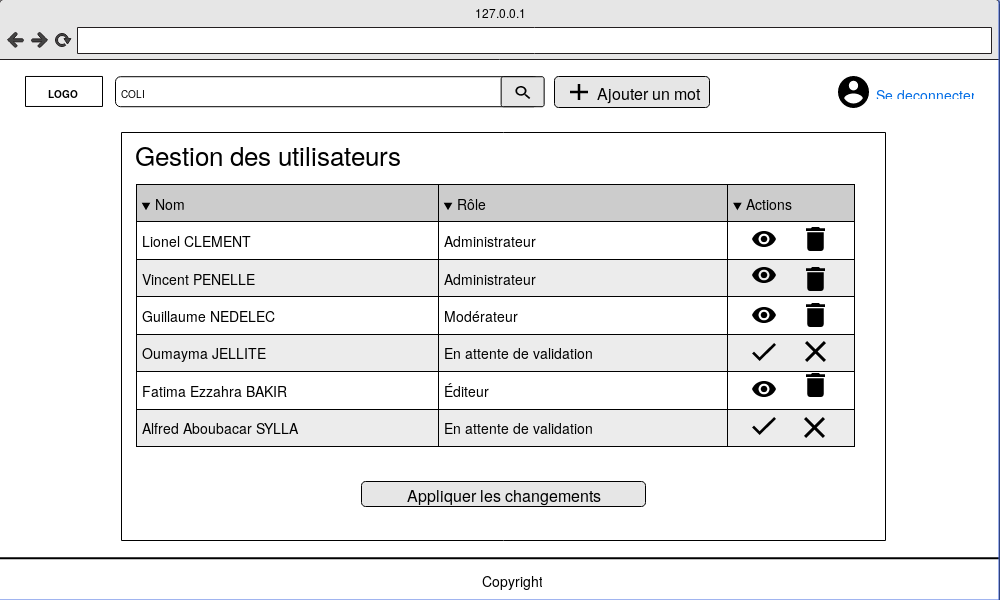
\includegraphics[width=150mm]{img/user_screen.png}\end{center}



\subsubsection{Gestion de l'historique d'un mot}
 \textbf{Priorité : 3} \\
Nous avons décidé de mettre en place un historique permettant d'enregistrer tous les ajouts, modifications et suppression. Pour cela nous voulons implémenter de l'Event Sourcing permettant d'enregistrer tous les évènements exécutés plutôt que d'enregistrer les données modifiées en base de données.
\subsection{Analyse des besoins non fonctionnels}
\smallbreak

\subsubsection{Sécurité}
\textbf{Priorité : 1}
\smallbreak
Afin de protéger l'intégrité des données du LeFFF dans la base de données, nous sécuriserons la base et l'application web des problèmes de sécurité suivants :
\begin{itemize}
    \item \textbf{Les injections SQL}, permettant de récupérer ou d'altérer des données, voir même prendre le contrôle de serveur. L'attaque par injection SQL consiste à injecter du code malicieux SQL qui sera interprété par le moteur de base de données dans un champ de saisie d'une application web. \\
    \textbf{Notre solution :} Afin de se protéger de se genre d'attaque, nous avons choisi de développer l'application web en PHP avec le framework Symfony, qui comprend un l'ORM (Object-Relational Mapping) Doctrine. Cet ORM est une couche d'abstraction de base de données qui permet d'interagir avec le contenu de la base de données en manipulant des objets (informatique) du coté de notre application. Il comprend des modules de sécurité (génération de contraintes, formatage des données envoyées ect...) qui détecte les attaques par injection SQL.
    
    \item \textbf{Le Cross-Site Scripting (XSS)} : Cette faille permet d'injecter du code malicieux sur une page web. Par exemple sur un forum, si quelqu'un entre en commentaire un code Javascript nuisible, tous les autres utilisateurs qui accéderont à cette page seront impacté par ce code qui s'exécutera sur leur navigateur. \\
    \textbf{Notre solution :}Pour remédier à cela, le framework Symfony possède aussi un système (filtrage des données d'entrées, échappement des données en sortie...) protégeant de ce genre d'attaque afin de filtrer tous ce qui pourrait ressembler à du code. C'est un procédé assez similaire à celui de la protection contre les injections SQL.
    
    \item \textbf{La falsification de requête inter-sites (CSRF)} : Cette faille permet à un attaquant de forcer ses victimes à effectuer certaines actions sur un site cible, sans qu’elles s’en aperçoivent. Pour cela, les attaquants cherche à ce que leur victime visite une page (en étant connecté) où des scripts malicieux seront exécutes sans que la victime s'en aperçoive à l'aide de balise image chargeant le script par exemple. La victime étant authentifié sur le site, les scripts pourront s'exécuter correctement et corrompre les données du site. \\
    \textbf{Notre solution :} Voici la dernière faille de sécurité à laquelle Symfony nous protège. En effet le framework fait cela en générèrant des jetons ("tokens") au moment de l'authentification, différents pour chaque utilisateur et qui sont stockés dans la session. Ce jeton est ensuite vérifié a chaque action avec la base afin de vérifier que c'est bien une action voulue par l'utilisateur et non une attaque CSRF. 
    
    \item \textbf{Le déchiffrement de données} qui consiste à déchiffrer des données crypté. Cela peut permettre de trouver des mot de passe et donc prendre le contrôle d'une session utilisateur ou bien de découvrir des informations sensibles (informations bancaire, personnelles...) \\
    \textbf{Notre solution :} Pour éviter cela, nous avons décidé de chiffrer les données avec des algorithmes irréversible (une fois crypté, aucune technique connue à ce jour peut décrypter le mot, il faut forcement connaître le mot initial) comme "bcrypt" ou "sha512".
    
    \item \textbf{L'écoute de communication réseau} : Requêter un site web avec un protocole HTTP permet à des intrus présent sur votre réseau de lire ou modifier le site internet que vous souhaitez consultez et présente donc un gros risque. \\
    \textbf{Notre solution} : Utiliser le protocole HTTPS qui permet de chiffrer les données échangées et ainsi les protéger de toutes interceptions ou modification.
\end{itemize}

\subsubsection{Format de fichier}
\textbf{Priorité : 2}
\smallbreak
\begin{itemize}
\item Afin de pouvoir répondre aux besoins d'importation et d'exportation du LeFFF avec la base de données, il nous faut définir les format de fichiers compatibles avec ces fonctions.
Nous avons fait le choix d'utiliser les formats textes et elex (.txt et .elex)  car ce sont les formats disponibles au téléchargement du LeFFF actuellement. Ce choix nous permet de pouvoir exploiter le LeFFF existant sans avoir à le reformatter dans un autre format.
\end{itemize}

\subsubsection{Performances}
\textbf{Priorité : 3}
\smallbreak
Au niveau des performances, nous avons décider de faire une implémentation du projet de manière à ce que la requête de demande des formes fléchies d'un mot (requête en base et génération des formes fléchies par le compilateur) n'excède pas les deux secondes d'exécutions. De plus les actions d'importation et d'exportation étant plus lourdes, nous voulons implémenter ces fonctions pour qu'elles n'excèdent pas 10 minutes d'exécution.

\subsubsection{Ergonomie}
\textbf{Priorité : 4}
\smallbreak
Nous avons fait le choix d'adopter une design très simple et épurée afin que l'utilisateur ne se perde pas dans l'interface et puisse trouver des solutions à son besoin de manière simple et naturelle.
\smallbreak
Des codes couleurs et icônes distinctifs seront mis en place afin que l'utilisateur comprennent le plus rapidement possible à quoi il est confronté. (par exemple, les messages en rouge correspondront à des messages d'erreurs, le vert pour la validation et du jaune pour des avertissements.).

\subsection{Contraintes}
\subsection{Solutions proposées : les besoins réalisés}

Après l'analyse des problèmes du système actuel, nous avons proposé la réalisation d'un site Web  adaptée aux besoins 
qui permettra d'améliorer le processus de travail et de gagner plus de temps en assurant :

\begin{itemize}
\item \textbf{La protection des données } : A l'aide d'une page d'authentification.
\item \textbf{Importations des fichiers} : Intégration à partir d'une interface graphique, le lexique qui existent dans l'archive du format texte.
\item \textbf{Exportations des fichiers} : Pour avoir une versions de lexique sous format texte.
\item \textbf{Recherche} : Pour avoir une versions de lexique sous format texte.
\item \textbf{Gestions des données} : d'une façon rapide et efficace et dans une seule interface graphique.


- L'ajout des mots, des règle, des combinaisons et des catégories.


- La modification et la suppression des mots, des règle, des combinaisons et des catégories.
\item \textbf{Possibilité du filtrage} : lors de la recherche dans les listes.
\item \textbf{Possibilité de la modification et suppression dans les listes.}
\end{itemize}
\section{Architecture et description du logiciel}
\subsection{Architecture de la base de données }

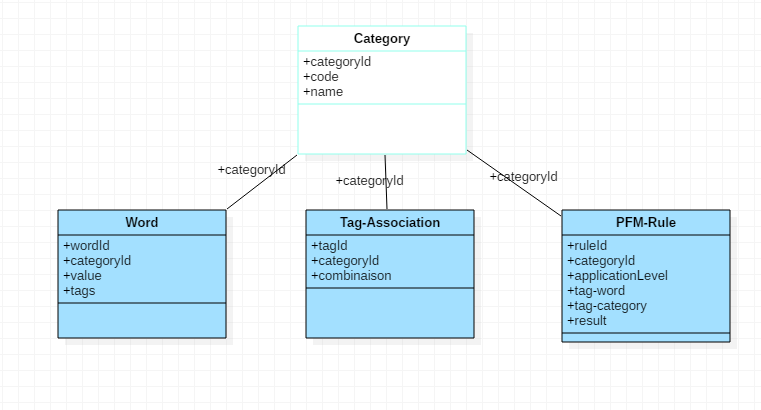
\includegraphics[width=150mm]{img/basefinal.PNG}

Notre base de données est constitue de quatre table : 
\begin{itemize}
\item \textbf{Category} : cette table contient le code et le nom de la catégorie ,par exemple code : adj et name : adjectif .
\item \textbf{Word} : la table word contient une référence categoryid vers la table category , la valeur du mot et ses tags (exp : groupe,etc).
\item \textbf{Tag-Association} :cette table contient des combinaisons de règles qui marche avec une catégorie renseignée par la clé étrangère CategoryId  et un tag du mot par exemple le groupe pour les verbes en français .
\item \textbf{PFM-Rule} : Nous avons choisi de stocker les règles PFM en base pour pouvoir les récupérer facilement par la suite et générer les formes fléchis d'un mot , en plus nous avons mis en place une interface pour que l'administrateur ou l'éditeur puisse ajouter des règles .

\end{itemize}
\subsection{Génération des formes fléchis  }
\subsubsection{Présentation du PFM }
L'interpréteur  nous permet de générer les formes fléchies d'un mot donné en entrée. 
Notre client nous a proposé PFM ( paradigm function morphology), selon cette approche , l'association d'un mot fléchi avec ses propriétés morphosyntaxiques permet d'appliquer des règles déterminant la forme flexionnelle de ce mot.


      Le format de base des régles : \textbf{n, Xc, t -> f(X) } \\
\begin{itemize}
    \item n : l’ordre de priorité pour l’application des règles
    \item X : la racine du lexème.
    \item C : la classe du lexème (sa catégorie).
    \item t : règles à appliquer
    \item f(X) : la forme flexionnelle
\end{itemize}

Exemple de règles pour les adjectifs : \\
\textbf{1, racine,{f} -> racine + "ne"} \\
\textbf{2, racine, {p}-> racine + "s"}

Exemple d'application : \\
PF(Sien, {f,p} ) = 2 o 1(Sien, {f,p} )(\textbf{ epsilon}) \\
                 = 2(Sien, {f,p} )(\textbf{ Sienne}) \\
                 =\textbf{ Siennes }

Pour cet exemple on veut mettre le mot sien au féminin pluriel ; la première règle à appliquer c'est d'ajouter le "ne" du féminin puis ajouter le "s" du pluriel en appliquant la deuxième règle ce qui nous assure l'ordre de priorité d'application des règles pour ne pas avoir des incohérences .
\subsubsection{Implémentation}


Nous avons choisi d'implémenter l'interpréteur en PHP.
Cet interpréteur, nous permet de générer les formes fléchies d'un mot.
En effet, Le rôle de l'interpréteur est important lors de la recherche d'un mot et l'exportation du lexique.
Pour la recherche du mot l'utilisateur doit données en paramétre le mot, 
dans un premier temps , on récupère les règles , les tags du mot et les combinaison de tags qui convient avec la catégorie du mot donnée en entrée, ensuite on filtre les règles selon la correspondances avec les tags du mot et on récupère aussi les règles définissant le radical du mot sachant que nous avons choisi de stocker pour chaque mot une règle qui définit son radical avec le formalisme PFM ,puis en vérifie si le tag du mot est renseigne dans les règles et si le mot en lui-même est un tag de la règle . 
Dans un deuxième temps on vérifie si tous les tags de la règle sont renseignes dans la combinaisons ou si aucun tag n'est renseigné ensuite on fait un tri des règles dans leur ordre d'application .
Pour l'application des règles on vérifie au début si la règle possède une combinaison de tags correspondant à une combinaison de tag de la catégorie si c'est le cas on l'applique, sinon on l'ignore en plus si plusieurs règles s'appliquent pour une combinaison données , elles respecte l'ordre croissant du niveau d'application , si le niveau est le même , la règle la plus spécifique avec le plus de tags qui correspondent s'applique et on ignore les autres .

\subsection{Outils de développement}

Ce projet est divisé en 3 parties :
\begin{itemize}  
  \item l'application web
  \item l'interpréteur
  \item la base de données
\end{itemize}

\textbf{Application web et L'intérpreteur : PHP avec le framework Symfony 4:}

Nous avons choisi de développer le site Web et l'interpréteur en PHP car c'est un langage simple d'utilisation et que ce framework apporte beaucoup d'avantages en termes de sécurité (comme énoncé précédemment dans la partie 2.2.1) et de développement (configuration simple et rapide ect...) ainsi, qu'il offre des 

\smallbreak

\textbf{Base de données : MySQL:}


Pour la base de données, le choix s'est porté sur MySQL pour sa facilité d'utilisation et sa bonne compatibilité avec le framework Symfony utilisé pour le site web. 


\textbf{Ces choix des outils ont des avantages énormes coté client:}

\begin{itemize}  
  \item solution client léger : Rien d'autre qu'un navigateur pour faire fonctionner l'application sur le poste de l'utilisateur.
  \item MySQL est très rapide : Puisque notre base de données contient un lexique très lourd l'accès aux données à l'aide de MySQl devient un peu plus rapide.
\end{itemize}

\subsection{ Architecture du Site Web }
\subsubsection{Schéma du site} 

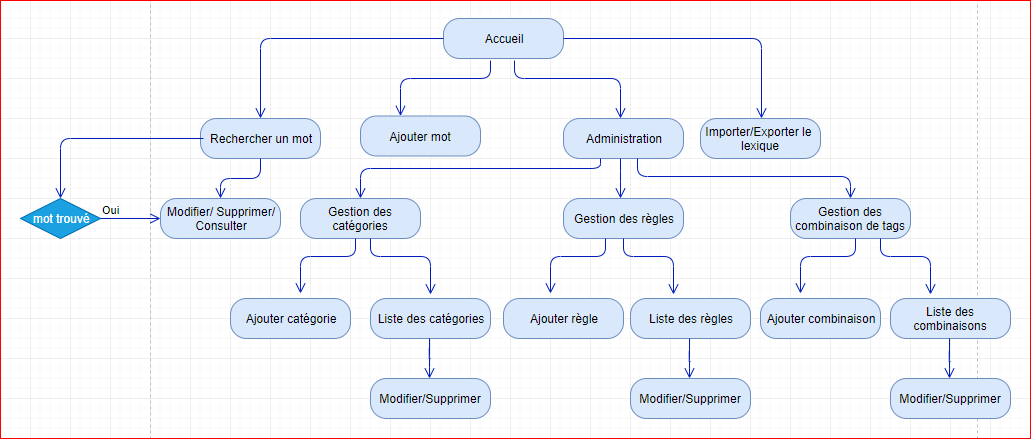
\includegraphics[width=150mm]{img/site.PNG}

Nous avons réussi à mettre en place les interfaces décrit dans le schéma ci-dessus,
Notre site web est réalisé seulement pour l'administrateur, qui doit s'authentifier
avant d'accéder aux différents services proposé par le site.

Cette interface permet aux utilisateurs de s'authentifier à l’aide d'un login et un Mot de passe, 
et faire la redirection vers la page d'accueil (dans notre application la page d'accueil
pour l'administrateur c'est le page de recherche d'un mot).

La recherche d'un mot consiste à afficher toutes les formes fléchies qui lui correspond. Une fois ces formes sont affichées, 
l'administrateur peut modifier le mot qu'il vient de rechercher.

La page d'accueil contient également des boutons qui redirigent vers les différents interfaces d'ajout : 
\begin{itemize}
    \item   Ajouter règle
    \item   Ajouter mot
    \item   Ajouter combinaison
    \item   Ajouter catégorie
   \end{itemize}
et elle redirige aussi aux  pages qui permet d'importer ou d'exporter le lexique.


\subsubsection{Exemple de bon fonctionnement: Interfaces} 

\begin{itemize}  
  \item Rechercher Mot
\end{itemize}
Les utilisateurs peuvent consulter la liste des formes fléchies du mot comme vous voyez dans cette interface :


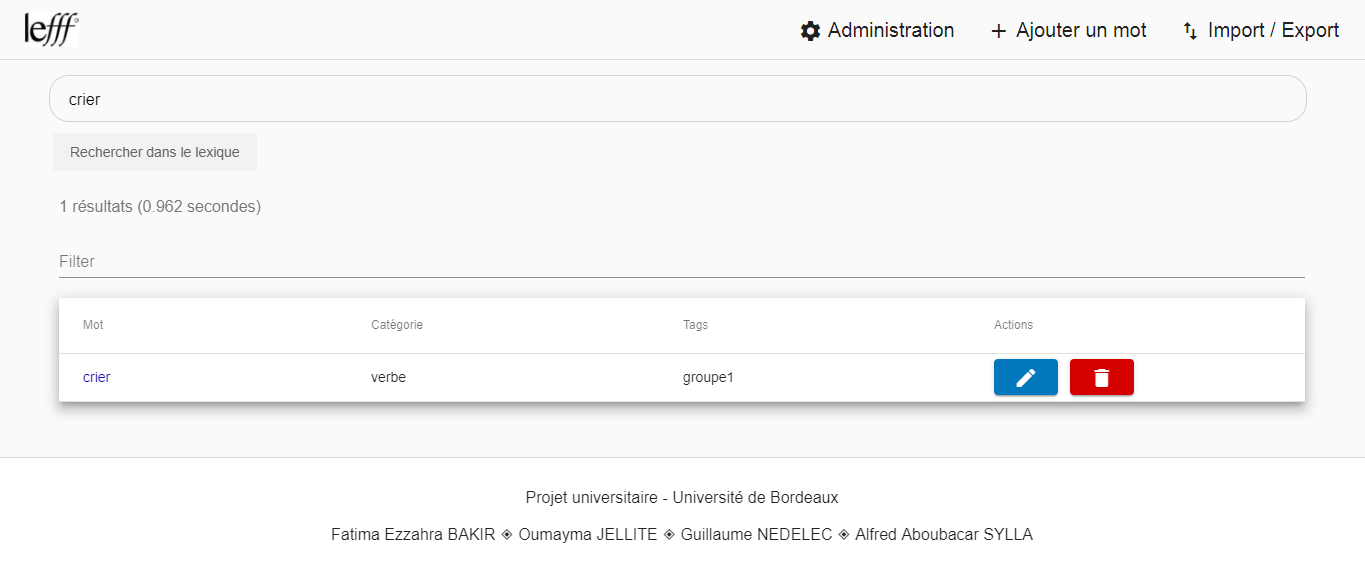
\includegraphics[width=150mm]{img/Recherche.PNG}



L’utilisateur (l’administrateur) peut gérer le mort en le modifiant ou le supprimer.


\begin{itemize}  
  \item Ajouter mot
\end{itemize}

L'administrateur a le droit d'ajouter des nouveaux mots  en accédant à l'interface suivante: 


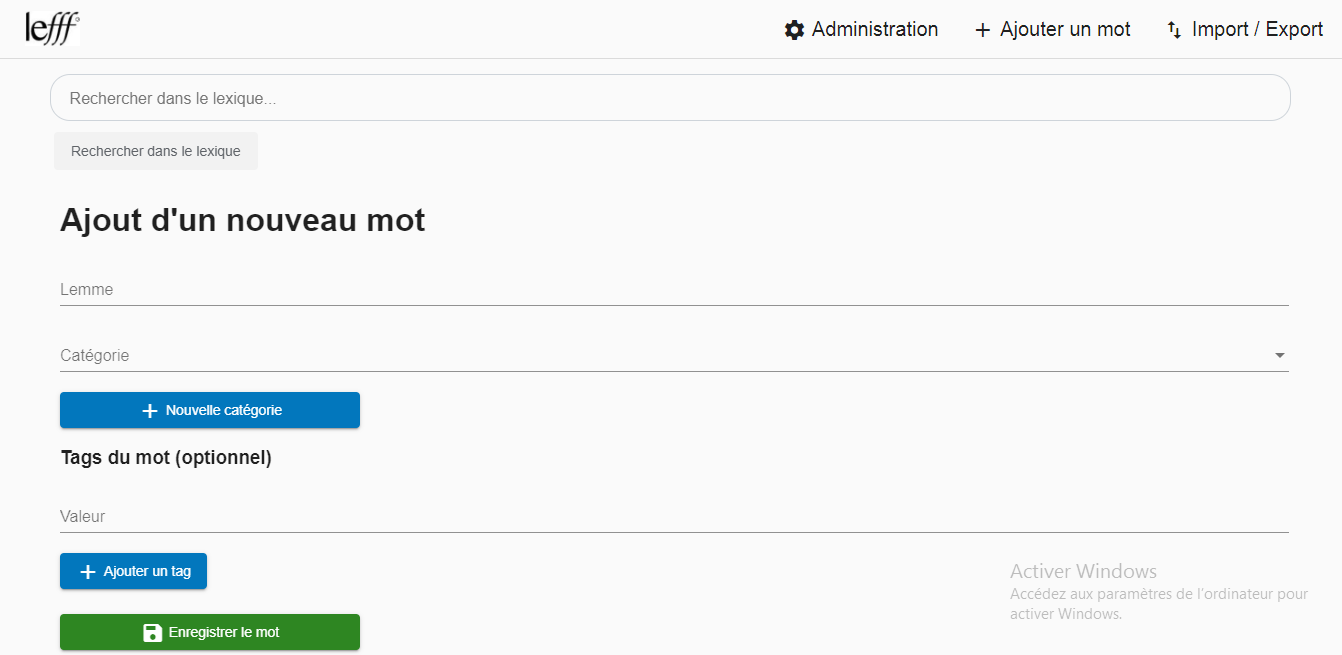
\includegraphics[width=150mm]{img/Ajoutermot.PNG}


Si le mot  est ajouté, un message de réclamation s'affiche. Une fois il est ajouté, l'utilisateur peut cliquer sur les boutons "Modifier" ou "Supprimer" si il a commis une erreur comme le montre la figure suivante:


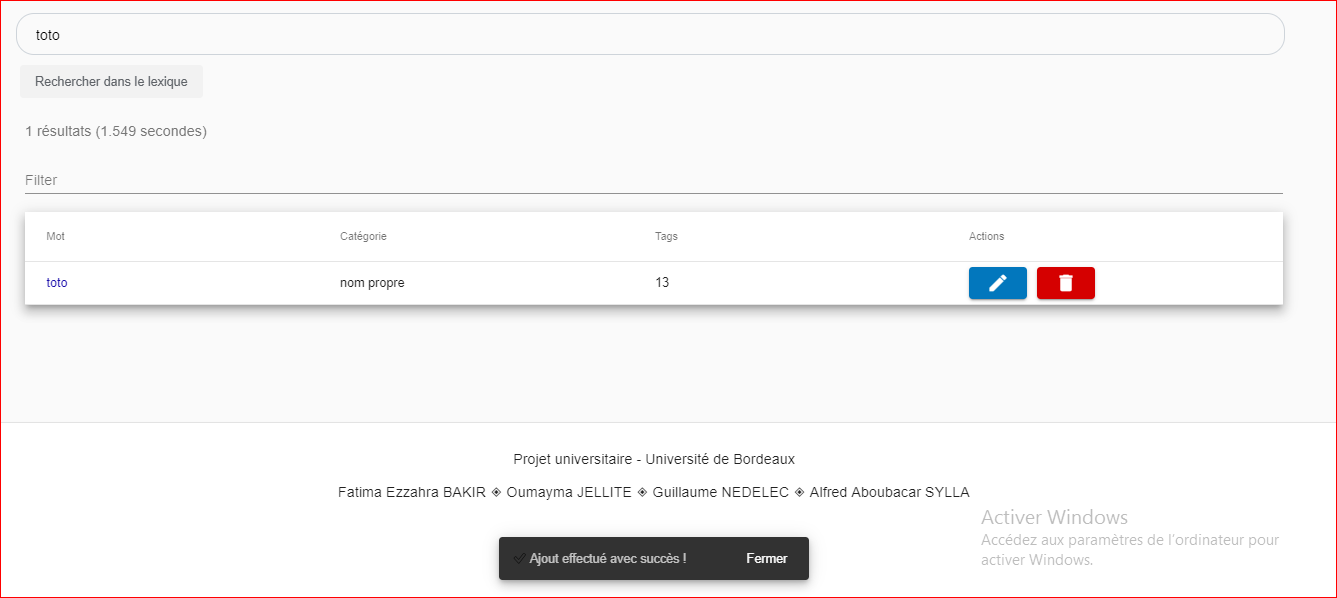
\includegraphics[width=150mm]{img/AjoutEffectuer.PNG}


\begin{itemize}  
  \item Modifier Mot
\end{itemize}
L'interface suivante nous permet de modifier les mots en affichant des messages de réclamation : 

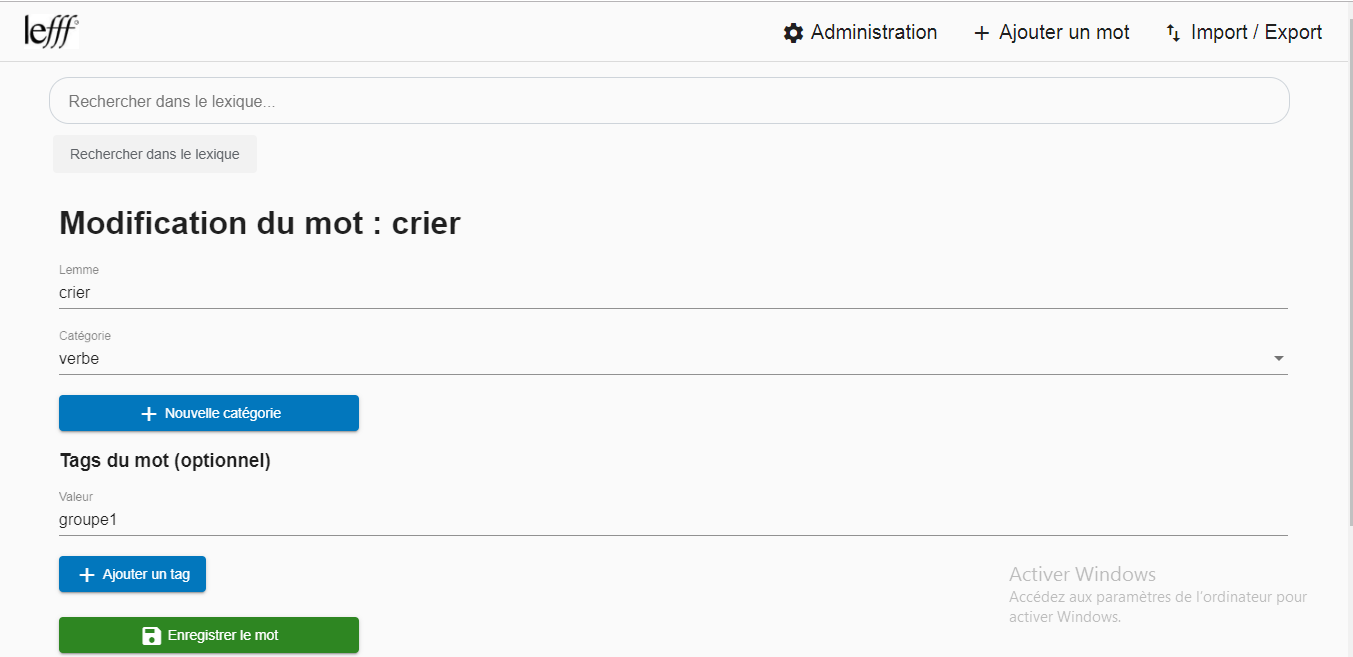
\includegraphics[width=150mm]{img/ModificationMot.PNG}


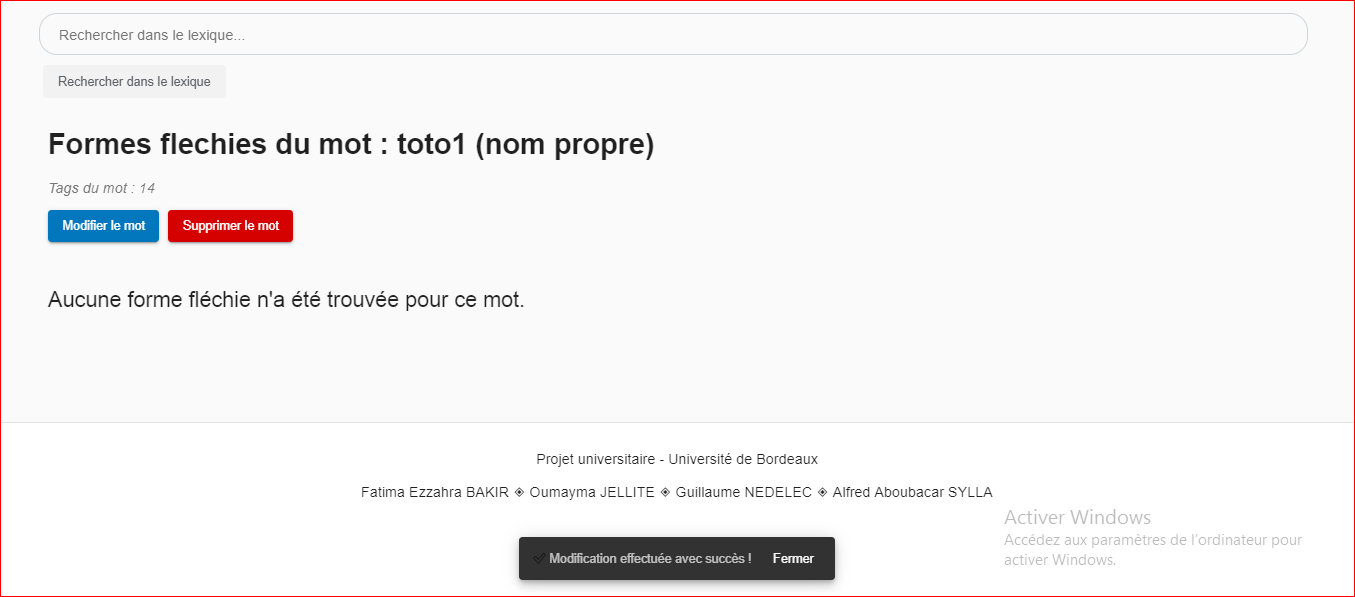
\includegraphics[width=150mm]{img/ModificationEffectuer.PNG}


\begin{itemize}  
  \item Supprimer Mot
\end{itemize}
Pour la suppression des mots, elle est possible comme il est montrer dans la figure suivante:

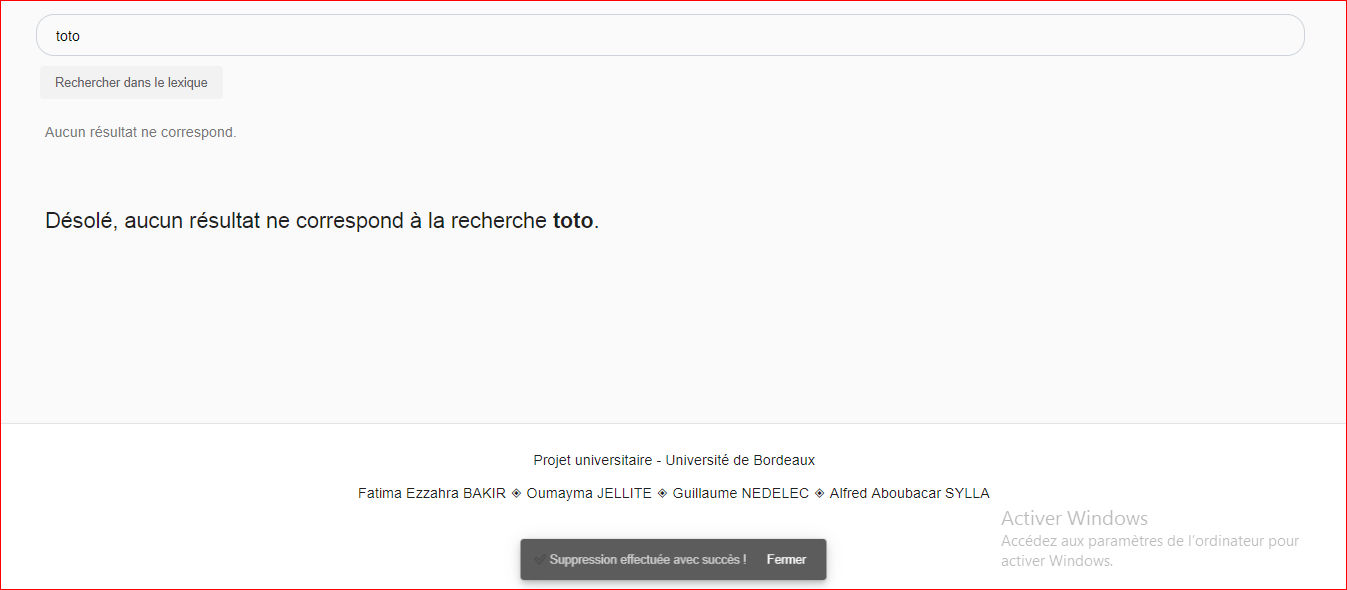
\includegraphics[width=150mm]{img/SuppressionEffectuer.PNG}


\begin{itemize}  
  \item Ajouter Catégorie / Ajouter Régle 
\end{itemize}

Notre site web, permet aussi l'ajout des catégories et des règles comme il est montré dans les figures ci-dessous: 


 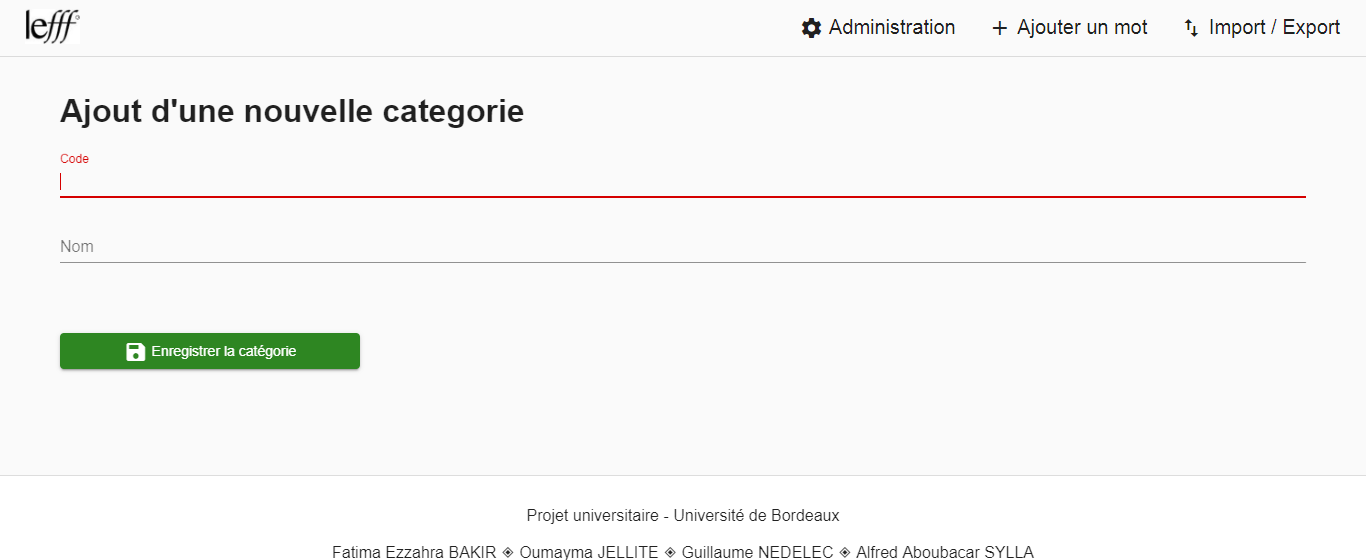
\includegraphics[width=150mm]{img/AjouterCat.PNG}


 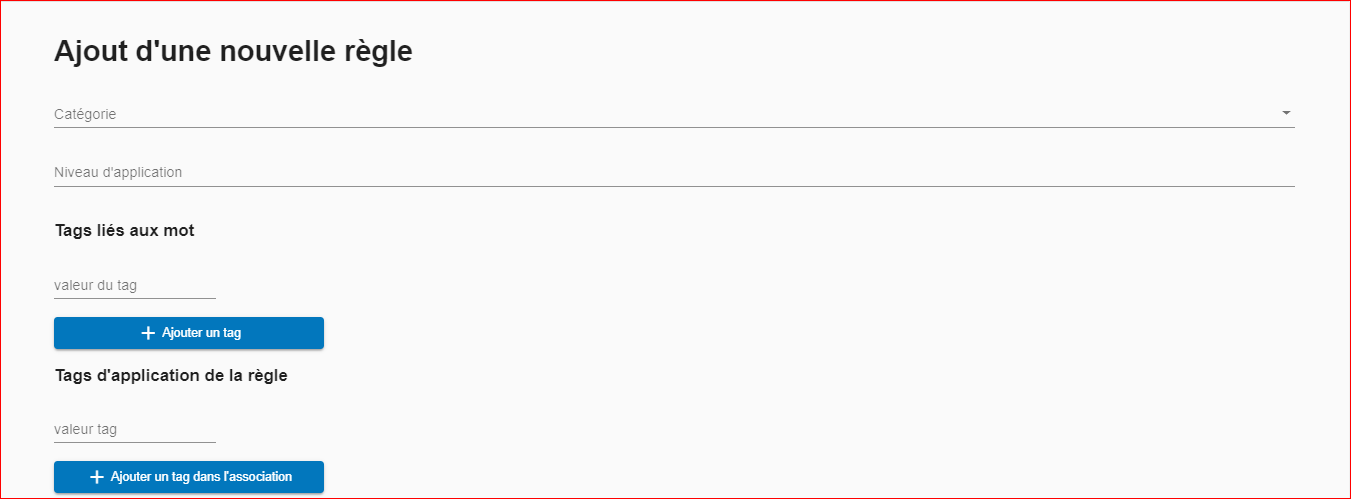
\includegraphics[width=150mm]{img/AjouterReg1.PNG}
 
 
 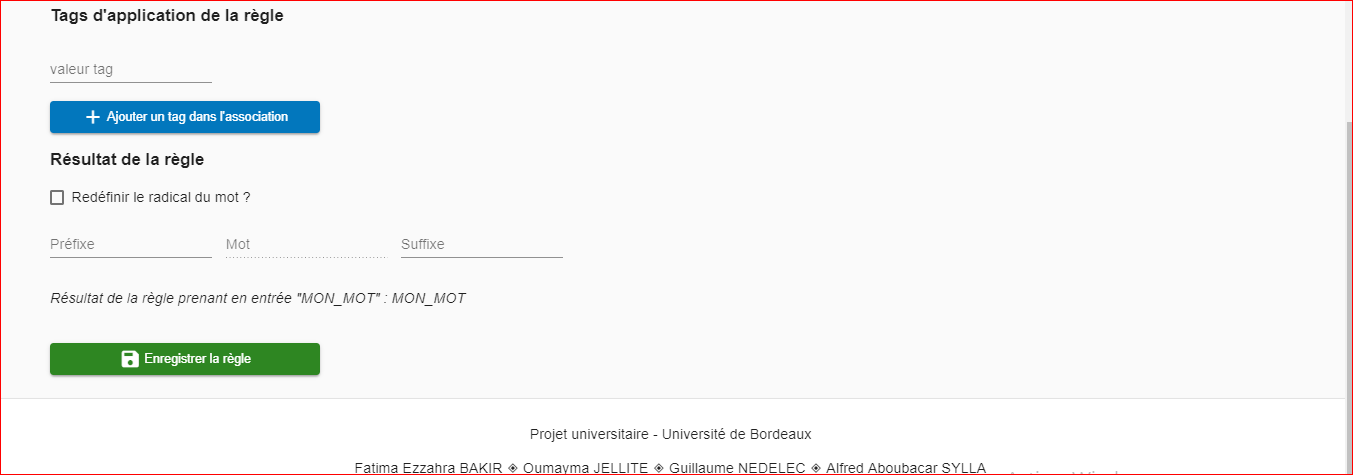
\includegraphics[width=150mm]{img/AjouterReg2.PNG}



\begin{itemize}  
  \item Listes des Catégories et des règles:
\end{itemize}
Les utilisateurs peuvent consulter la liste des règles et des catègories dans les pages correspondante comme les montres les figures ci-desous: 


 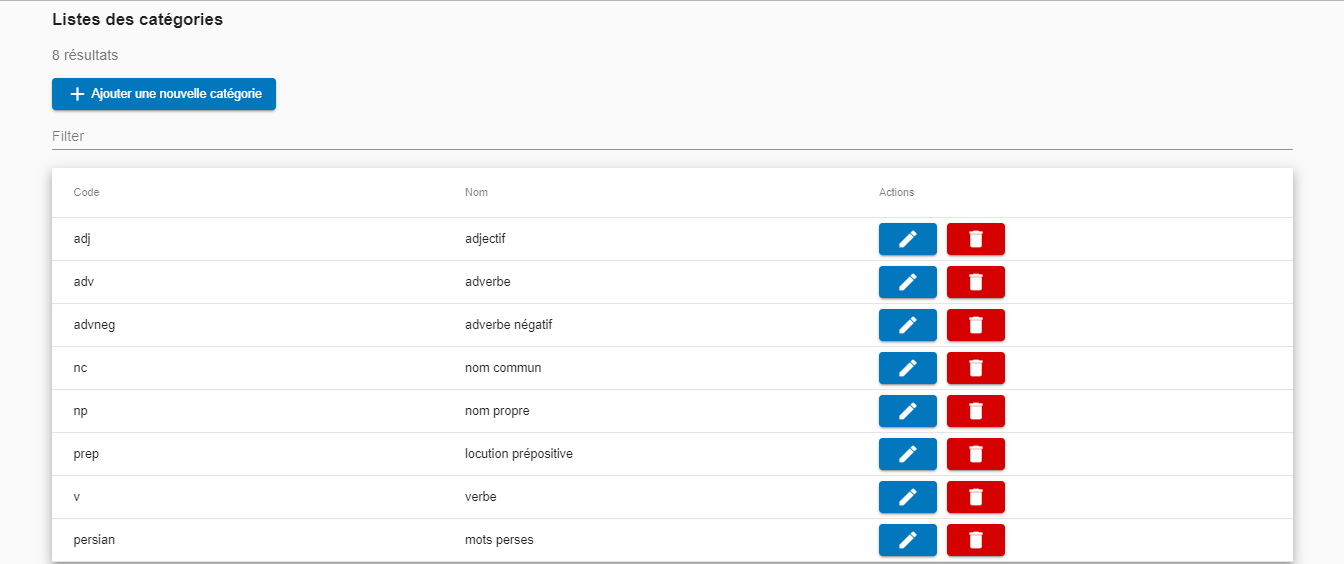
\includegraphics[width=150mm]{img/GestionCat.PNG}


 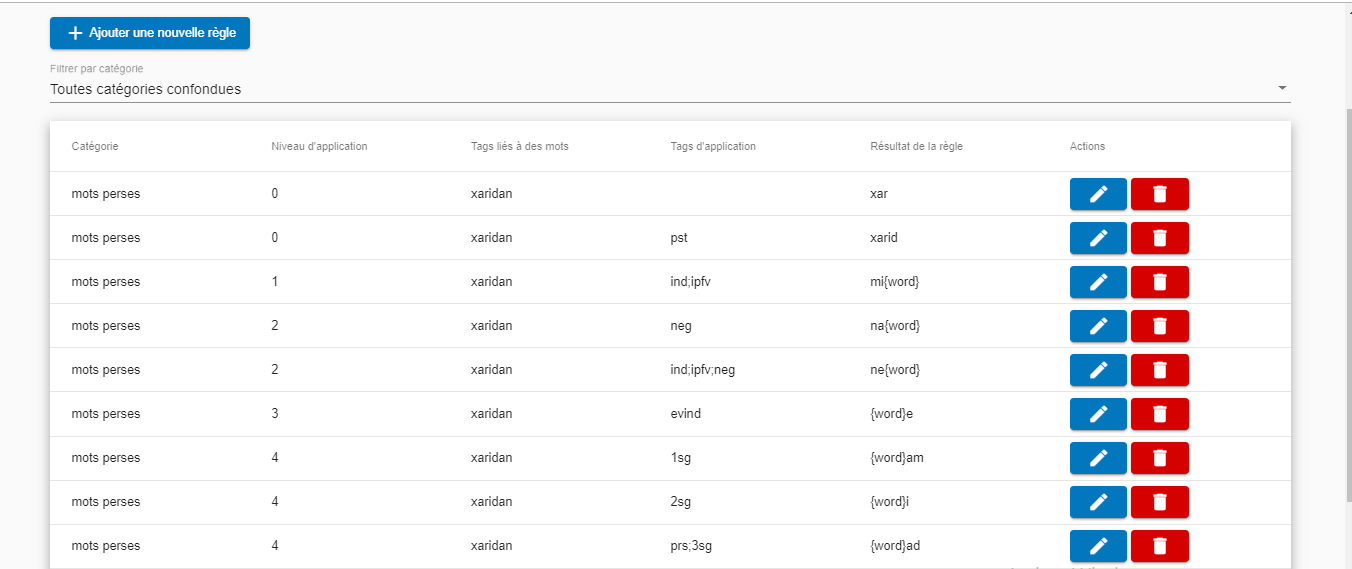
\includegraphics[width=150mm]{img/GestionReg.PNG}


Ces pages, permet aux utilisateurs  d'effectuer plusieurs fonctionnalités: La consultation, la modification et la suppression.




\begin{itemize}  
  \item Exporter le lexique
\end{itemize}
Les utilisateurs peuvent aussi exporter le lexique en extrayant tous les mots enregistrés en base de données dans l'ordre alphabétique avec leurs formes fléchies générer par l'interpréteur :

 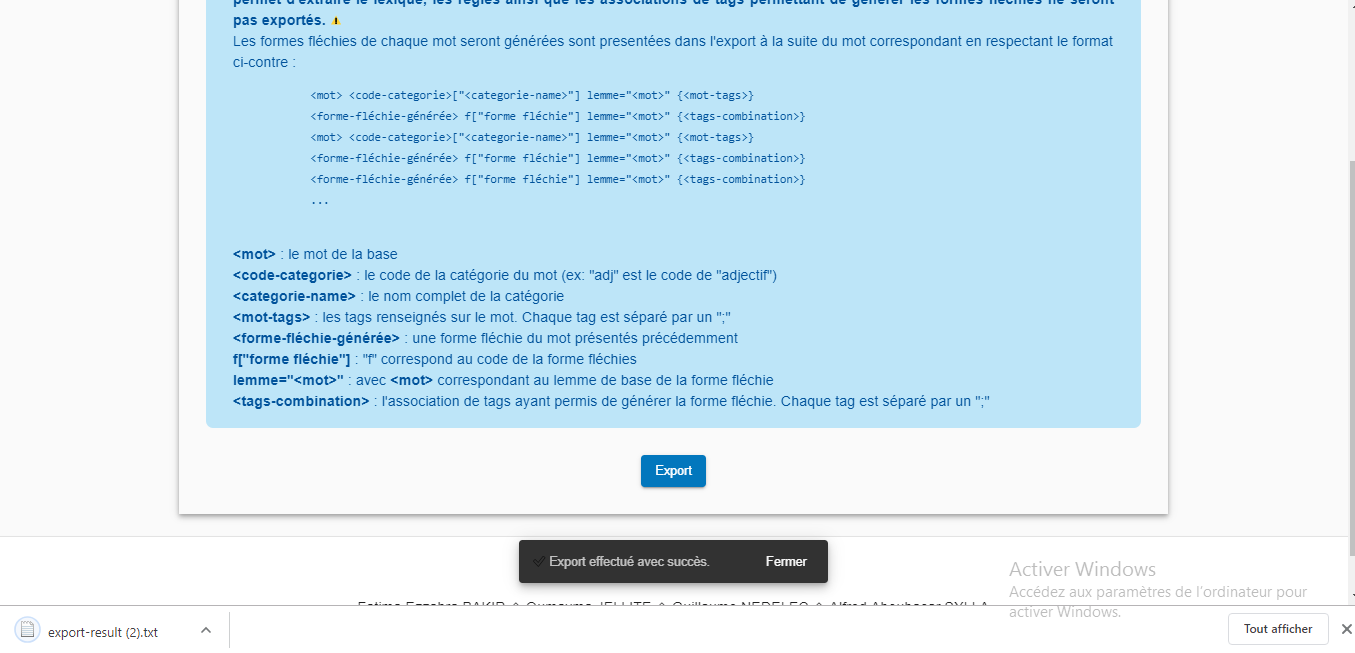
\includegraphics[width=150mm]{img/ExportReussi.PNG}


 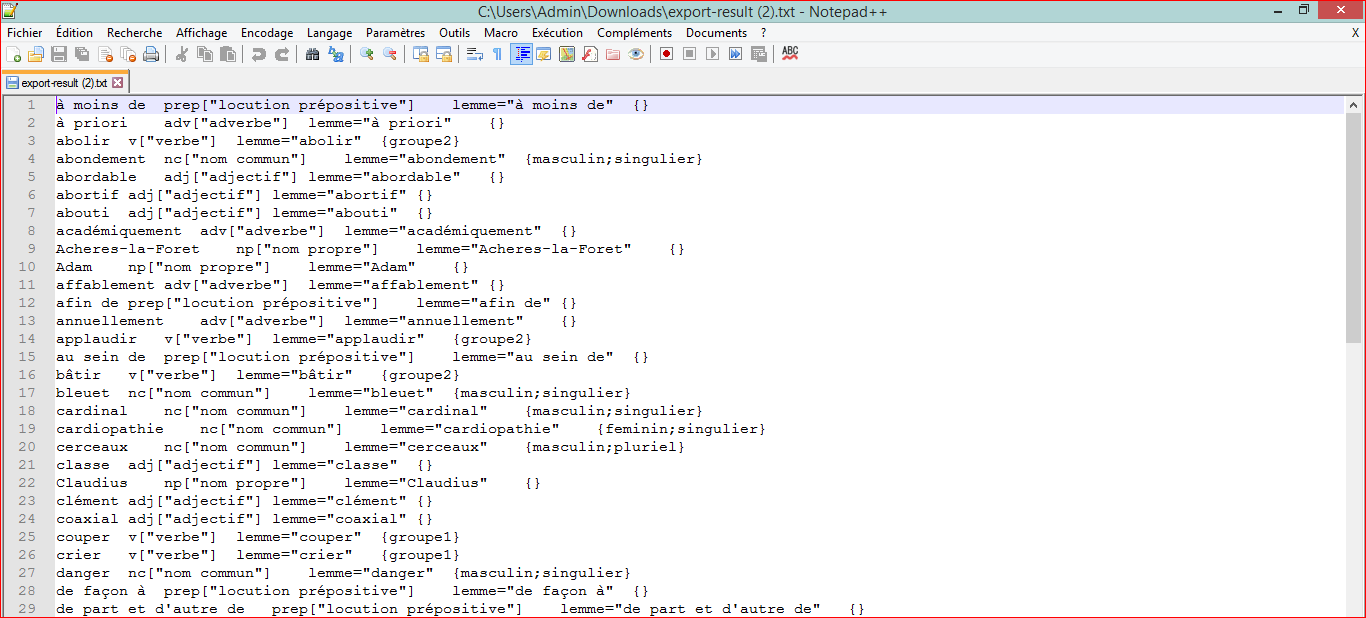
\includegraphics[width=150mm]{img/ExportTxt.PNG}

\begin{itemize}  
  \item Importer le lexique
\end{itemize}
ON a ajouté une interface ou les utilisateurs peuvent importer les fichier sous format texte qui existent déjà. Pour cela on a définie 3 syntaxes différentes : 


La  première correspond à celle respectée par notre fonctionnalité d'export.




La deuxième  correspond à la syntaxe du Lefff consultable le site de Lionel CLEMENT.



Et La troisième  correspond à la syntaxe du Lefff au format .mlex consultable sur le site de Benoît SAGOT..

						


\section{Analyse du fonctionnement et tests}

\section{Conclusion}

Notre objectif de ce projet de programmation était de concevoir et d'implémenter un site Web pour la gestion des formes fléchies.
Ce site Web est une évolution importante qui a permis de mettre fin à la majorité des problèmes et des insuffisances de la gestion des formes fléchies sur les documents format texte. 


Après une profonde méditation, on a fait une présentation du contexte général du projet et ses aspects. C'est-à-dire comprendre le fonctionnement de la génération des formes fléchies, les lacunes ou insuffisances du système actuel et les besoin, pour faciliter le déroulement du site Web à la deuxième étape. 
La dernière étape consiste la mise en œuvre pour adapté un système
adéquat avec les différents outils et langages utilisés dans le développement de notre application.

Ce projet nous a permis d'enrichir nos connaissances dans le monde de développement des site Web, mettre en pratique une partie des connaissances acquises lors de notre formation universitaire et de notre auto-formation dans des domaines très variés comme :  Symphonie, Angular ...
 

En termes d'évolution, l'application « Le Clicodrome de LEFFF » pourra par la suite être finalisée et adaptée au client.
En ajoutant les fonctionnalités qu'on a pas réussi à les implémenter faute de temps: Comme la gestion des utilisateurs.En effet, chaque utilisateur de notre système doit avoir des rôles bien spécifiques, aussi la gestion des historiques pour garder trace de chaque modification apportée au lexique.

L'apport de ce travail a constitué une occasion pour nous immerger dans le monde professionnel et appréhender la réalité des métiers de développement, conception et de gestion des projets et apprendre à organiser des réunions professionnelles avec le client et l'équipe. En effet l'expérience acquise durant ces deux mois est précieuse pour nos futures carrières professionnelles.
\section{Références}
\bibliography{references}
\bibliographystyle{plain}
\end{document} 